\chapter{Introducción}
\label{chapter:introduccion}


%%% SECTION
\section{Descripción general del problema}

% Descripción general del problema~\cite{webscraping}.
En la actualidad, abundan las ofertas de financiación y apoyo económico promovidas por organismos tanto públicos como privados. 
Sin embargo, las organizaciones empresariales encuentran dificultades para determinar qué oportunidades realmente se ajustan a su perfil específico. 
El gran caudal de datos y su heterogeneidad crean un panorama confuso, agravado por la carencia de sistemas automatizados que faciliten una búsqueda eficiente.

Entre las dificultades no solo se encuentra el hallazgo de convocatorias apropiadas, sino también entender la documentación requerida, los cronogramas de presentación, y determinar si estas ayudas son realmente aplicables al contexto empresarial particular. 
Adicionalmente, las compañías deben gestionar información fragmentada y frecuentemente desorganizada distribuida en múltiples fuentes digitales, lo que incrementa la complejidad del proceso de filtrado y selección.

Este proyecto plantea una solución que agilize, simplifique y optimice este proceso de búsqueda de financiación. 
Mediante la combinación de tecnologías como Inteligencia Artificial Generativa \cite{iag}, Procesamiento de Lenguaje Natural (NLP) \cite{Khurana_2022} y métodos de extracción de datos web o scraping \cite{webscraping}, es posible extraer información precisa, relevante y estructurada sobre la documentación de estas convocatorias.

La importancia de esta solución se encuentra en su potencial para reducir tiempos y aumentar la efectividad al elegir opciones de financiamiento adecuadas. 
El hecho de implementar una solución como esta influirá positivamente en las tasas de éxito de las solicitudes presentadas y en la consecución de recursos económicos. 
El propósito de esta solución es democratizar el acceso a oportunidades financieras, fomentando condiciones más favorables para el desarrollo y la continuidad de las empresas.

\newpage

\section{Explicación de la motivación personal}

La motivación tras este proyecto nace del interés personal sobre el uso de las nuevas tecnologías, especialmente la Inteligencia Artificial, en aspectos de la vida, tanto personales como profesionales, donde pueden suponer un cambio importante en la forma de realizar ciertas tareas: Agilizando procesos, reduciendo la dificultad en algunos casos y, en resumen, facilitar y hacer más accesible ciertos aspectos de la vida personal y profesional que pueden resultar tediosos.

El uso de tecnologías como el Procesamiento de Lenguaje Natural y la Inteligencia Artificial Generativa están cambiando desde hace unos años nuestra tecnología a un ritmo nunca visto. Prácticamente cada pocos meses aparecen nuevas tecnologías basadas en este campo de conocimiento, pasando por nuevos Grandes Modelos del Lenguaje como GPT-4o o DeepSeek, nuevas herramientas de desarrollo como Langchain, LLamaIndex, u Ollama, e incluso aplicaciones basadas en IA como Cursor, NotebookLM, o diferentes aplicaciones que te permiten generar texto, imágenes o música sin ser un experto.

Todas estas tecnologías están cambiando la forma en la que vemos el mundo, y aunque es necesario cierto control y regulación para no acabar en unos años en una sociedad distópica digna de la ciencia ficción, sí que considero que tenemos que aprovechar el potencial de estas tecnologías para seguir el camino hacia una sociedad más justa, equitativa, y donde tenga más peso la calidad de nuestras vidas y los derechos sociales, que las obligaciones económicas y laborales que marcan nuestro día a día.

En este caso concreto del proyecto, el uso de estas técnicas permite democratizar y hacer más accesible este tipo de ayudas. Crear una empresa y mantenerla a flote no es fácil, y en muchos casos sólo unas pocas sobreviven más de unos pocos años tras su creación, generalmente porque parten de unas capacidades económicas por detrás que no disponen el resto. Este tipo de ayudas económicas permiten a empresas con menos recursos de partida salir adelante, y herramientas como estas facilitan la búsqueda y su participación en éstas.

\newpage

\section{Definición de los objetivos}

\subsection{Objetivo Principal}

El objetivo principal de este proyecto es el desarrollo de una solución automática basada en Inteligencia Artificial Generativa, que permita la indexación de información a partir de unas fuentes de datos concretas, en este caso convocatorias de ayudas a empresas, y realice tareas de extracción y estructuración de la información. 
De esta forma, se generará un barrido de todas las posibles convocatorias y se generará una base de datos con información relevante para su consulta y explotación.


\subsection{Objetivos Específicos}

\begin{itemize}

\item \textbf{Implementación de una herramienta de extracción de información}:\\
En primer lugar se diseñará una herramienta que sea capaz de identificar las diferentes convocatorias de ayudas a partir de las fuentes disponibles y extraer la información necesaria:
\begin{itemize}
    \item Codigo fuente de la página web de convocatorias.
    \item Ficha técnica de las convocatorias.
    \item Documentos asociados.
\end{itemize}
Esta herramienta será una combinación de soluciones basadas en Inteligencia Artificial Generativa y Web Scraping.

\item \textbf{Sistema NLP de extracción y procesado de información}:\\ 
Una vez extraída la información de la convocatoria, se emplearán diferentes técnicas de Procesamiento de Lenguaje Natural para diferentes tareas de procesado de texto y extracción de información. 
Este sistema empleará Grandes Modelos del Lenguaje (LLMs) en combinación con diferentes frameworks de orquestación, como Langchain o LLamaIndex.
Se emplearán diferentes propuestas de LLMs para evaluar su eficacia en la extracción de información.

% opcional si da tiempo
\item \textbf{Herramienta de consulta de información}:\\
Finalmente, se implementará una solución de consulta y recuperación de información sobre las diferentes convocatorias, partiendo tanto de los datos estructurados generados en el paso anterior como de las fuentes originales de datos.
Esta solución se basará en un RAG multiagente, empleando técnicas avanzadas en cuanto a Question Answering y procesamiento de texto.
\end{itemize}

\newpage

\section{Descripción de la metodología empleada en el desarrollo del proyecto}

En este proyecto, se ha optado por implementar la metodología Agile debido a su enfoque iterativo y flexible, lo que nos permitirá adaptarnos rápidamente a cambios en los requisitos y mejorar continuamente el resultado a través de entregas incrementales. 
Agile fomenta la colaboración, la comunicación y la retroalimentación continua, asegurando que el desarrollo se mantenga alineado con las necesidades del proyecto. 
Además, esta metodología promueve la eficiencia y la optimización del tiempo, reduciendo riesgos y mejorando la calidad del resultado final.

\begin{itemize}
\item \textbf{Estrategia de investigación}\\
La estrategia de investigación sigue el enfoque propuesto por Oates en su libro \textit{Researching
Information Systems and Computing} \cite{Oates2005ResearchingIS}, combinando técnicas de análisis de datos cualitativos
y cuantitativos para asegurar una comprensión holística del dominio.
Durante el proyecto, se aplicarán estrategias presentadas en el enfoque anterior para la obtención de datos de las convocatorias.
Las principales tecnologías empleadas en el desarrollo serán Python como lenguaje de programación, frameworks como Langchain, LLamaIndex o HuggingFace, y diferentes librerías de NLP y Web Scraping, así como diferentes Grandes Modelos del Lenguaje, algunos explotados desde su propia API, y otros desde orquestadores locales, como Ollama o LMStudio.
    
\item \textbf{Fases del desarrollo}\\
El proyecto se dividirá en diferentes fases, cada una de las cuales se centrará en una tarea específica.
    
\begin{itemize}
    \item \textbf{Fase de investigación}:
    Revisión y análisis des las fuentes de datos disponibles, que en este casos son las diferentes webs proporcionadas de convocatorias de ayudas.
    A partir de los datos disponibles en éstas, se podrán definir los requisitos y funcionalidades que tiene que tener el sistema en cuanto a ectracción y procesado de información.
        
    \item \textbf{Desarrollo de la herramienta de identificación y extracción de convocatorias}:
    En esta fase se desarrollará la herramienta de extracción de datos de convocatorias. Esta herramienta empleará una combinación de web scraping e IA Generativa para acceder a los sitios web de las ayudas, identificar las diferentes convocatorias y extraer las fuentes de datos en formato textual.

    \item \textbf{Desarrollo del sistema de procesamiento}:
    Una vez extraída la información, se desarrollará un sistema de procesamiento basado en IA Generativa que permita la identificación y extracción de información relevante de las convocatorias.
    Por un lado, extraerá datos en formato de texto web, que será procesado para cer accesible mediante Grandes Modelos del Lenguaje. Por otro lado, también procesará los ficheros PDF generalmente asociados a estas convocatorias.
    como resultado, se generará una base de datos con información estructurada, y una base de datos vectorial que almacenará los embeddings de los documentos.
    \item \textbf{Desarrollo del sistema de consulta de información}:
    A partir de las bases de datos generadas en el paso anterior, se construirá un sistema basado en RAG que permita acceder a esas fuentes y realizar consultas sobre los datos.
    Esas consultas permitirán extraer información estructurada en el formato solicitado.
    
\end{itemize}


\end{itemize}

\newpage

\section{Planificación o plan de investigación del proyecto}

El plan de desarrollo de este proyecto va marcado por las diferentes etapas que establece la metodología de la UOC.
En cada una de esos bloques de trabajo se abordarán las diferentes etapas indicadas del proyecto:

\begin{itemize}
    \item \textbf{19/02/2025 al 09/03/2025}:
    Definición del TFM: Enunciado y entrega (M1).
    Definición de los requisitos del proyecto, análisis de fuentes de datos y tecnologías disponibles.
    \item \textbf{10/03/2025 al 30/03/2025}:
    Estado del Arte: Enunciado y entrega de la actividad (M2). 
    En este bloque de trabajo se redactará el capítulo del Estado del Arte, en base a un trabajo de investigación donde se recopilarán las herramientas y tecnologías con potencial de ser empleadas en el proyecto.
    Este capítulo principalmente recopilará los últimos avances en Inteligencia Artificial Generativa, Grandes Modelos del Lenguaje, y frameworks asociados.
    Paralelamente comenzará el desarrollo de la herramienta de identificación y extracción de convocatorias.
    \item \textbf{31/03/2025 al 04/05/2025}:
    Implementación: Enunciado y entrega de la actividad (M3).
    Implementación de los diferentes bloques ya definidos: Herramienta de identificación de convocatorias, Sistema de procesamiento y la solución de consulta de información.
    \item \textbf{05/05/2025 al 18/05/2025}:
    Redacción de la memoria: Entrega preliminar (M4).
    \item \textbf{19/05/2025 al 25/05/2025}:
    Redacción de la memoria: Entrega final (M4).
    \item \textbf{26/05/2025 al 03/06/2025}:
    Presentación audiovisual del trabajo (M4).
    \item \textbf{04/06/2025 al 06/06/2025}:
    Entrega de la documentación al tribunal (M5).
    \item \textbf{07/06/2025 al 27/06/2025}:
    Defensa pública del trabajo (M5).
\end{itemize}

\begin{figure}[h]
	\centering
	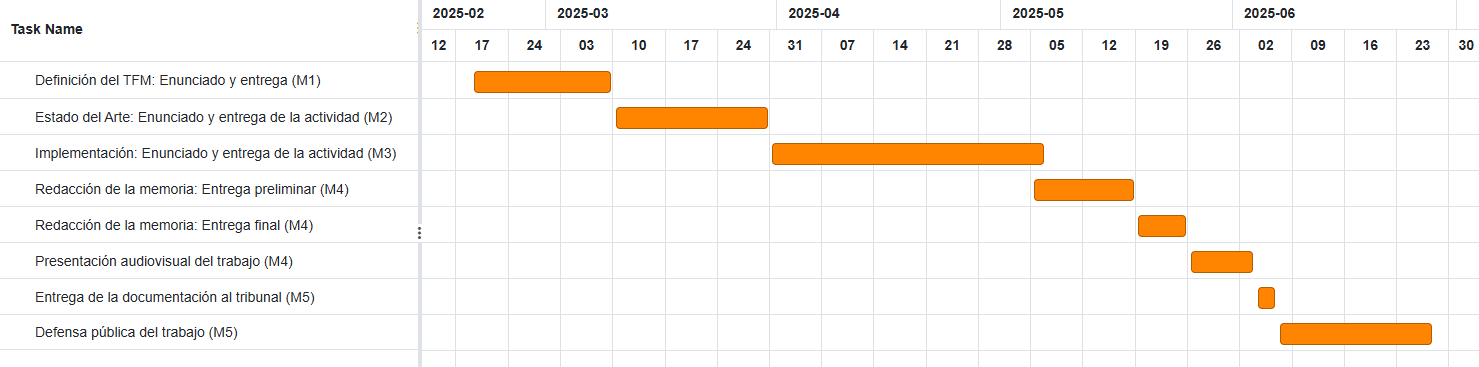
\includegraphics[width=0.9\textwidth]{figs/gantt.png}
	\caption{Timeline de tareas}
	\label{fig:context-anoni1}
\end{figure}

